% This text is proprietary.
% It's a part of presentation made by myself.
% It may not used commercial.
% The noncommercial use such as private and study is free
% Sep. 2005 
% Author: Sascha Frank 
% University Freiburg 
% www.informatik.uni-freiburg.de/~frank/
% additional use of \usepackage{beamerthemesplit}
\documentclass[usenames,dvipsnames]{beamer}
\usecolortheme{orchid}
%\usepackage[dvipsnames]{xcolor}
\usepackage{beamerthemesplit} % new 
\usepackage{tikz}
\usepackage{amssymb}
\usepackage{amsmath}
\usepackage{dsfont}
\usepackage{pifont}% http://ctan.org/pkg/pifont
\usepackage[T1]{fontenc}
\uselanguage{italian}
\usetikzlibrary{arrows.meta}
\usepackage{menukeys}
\usepackage{etoolbox}
\usepackage{movie15}
%\usepackage{graphicx}
\usepackage{sidecap}
\languagepath{english}


\usefonttheme[onlymath]{serif}
\deftranslation[to=italian]{Theorem}{Teorema}
\usetheme{CambridgeUS}




%\usepackage[inline]{enumitem}   



\definecolor{B}{RGB}{52,116,103}
\definecolor{greenx}{RGB}{80,100,0}
\definecolor{Gre}{RGB}{120,100,25}
\definecolor{darkred}{rgb}{0.8,0,0}
\definecolor{Brown}{RGB}{100,35,25}
\definecolor{baige}{RGB}{189,110,69}

\tikzstyle{hp} = [draw=Bittersweet, thick, rectangle, rounded corners, inner ysep=2pt, inner xsep=5pt]

\tikzstyle{th} = [draw=RedOrange, darkred, rectangle, rounded corners, inner ysep=2pt, inner xsep=5pt]

\tikzstyle{ot} = [draw=baige, thick, rectangle, rounded corners, inner ysep=2pt, inner xsep=5pt]

\tikzset{
	center coordinate/.style={
		execute at end picture={
			\path ([rotate around={180:#1}]perpendicular cs: horizontal line through={#1},
			vertical line through={(current bounding box.east)})
			([rotate around={180:#1}]perpendicular cs: horizontal line through={#1},
			vertical line through={(current bounding box.west)});}}}

\makeatletter

\setbeamercolor{block body example}{fg=black,bg=Gre!3!white}
\setbeamercolor{block title example}{fg=white,bg=Gre}

\setbeamertemplate{frametitle}[default][center]

\setbeamertemplate{theorem begin}{%
	\setbeamercolor{block title}{fg=white,bg=baige}%
	\setbeamercolor{block body}{fg=black,bg=baige!3!white}
	\setbeamercolor{itemize item}{fg=baige}%
	\setbeamercolor{itemize subitem}{fg=baige}%
	\setbeamercolor{itemize subsubitem}{fg=baige}%
	\setbeamercolor{enumerate item}{fg=baige}%
	\setbeamercolor{enumerate subitem}{fg=baige}%
	\setbeamercolor{enumerate subsubitem}{fg=baige}%
	\begin{\inserttheoremblockenv}
		{%
			\centering %\inserttheoremname
			%\inserttheoremnumber
			\ifx\inserttheoremaddition\@empty\else\ \inserttheoremaddition\fi%
		}%
		\normalfont%
	}
	
	\setbeamertemplate{theorem end}{%
	\end{\inserttheoremblockenv}%
}

\setbeamercolor{block body}{fg=black,bg=baige!5!white}
\setbeamercolor{block title}{fg=white,bg=baige}

\newcommand{\deftitle}[1]{\color{darkred}\bf{#1}\color{black}}
\newcommand{\dftitle}[2]{\color{#2}\bf{#1}\color{black}}
\newcommand{\cmark}{\ding{51}}%
\newcommand{\xmark}{\ding{55}}%
\newcommand{\N}{\mathbb{N}} % \N   = numeri naturali
\newcommand{\Z}{\mathbb{Z}} % \Z   = numeri relativi
\newcommand{\Q}{\mathbb{Q}} % \Q   = numeri razionali
\newcommand{\R}{\mathbb{R}} % \R   = numeri reali
\newcommand{\C}{\mathbb{C}} % \C   = numeri complessi
\newcommand{\F}{\mathbb{F}} % \C   = campo finito
\newcommand{\p}{\mathbb{P}}
\newcommand{\E}{\mathbb{E}}
\newcommand{\V}{\mathbb{V}}
\newcommand{\Ideona}{\color{YellowOrange!60!RawSienna}{Idea}\color{black}}

\newcommand{\ball}{
	\begin{tikzpicture}
		\node[circle,fill=darkred!60!RawSienna,inner sep=1.2pt, scale=2.5] { };
	\end{tikzpicture}
}

\setbeamertemplate{itemize item}{\ball}
\setbeamertemplate{itemize subitem}{\ball}

\setbeamertemplate{enumerate item}{\ball}
\setbeamertemplate{enumerate subitem}{\ball}

\newcommand{\palla}[1]{
	\begin{tikzpicture}
		\node[circle,fill=darkred!60!RawSienna,inner sep=2pt, scale=1.5] {#1};
	\end{tikzpicture}
}

\newcommand{\pall}[1]{
	\begin{tikzpicture}
		\node[circle,fill=#1,inner sep=2pt, scale=1.6] { };
	\end{tikzpicture}
}


% Patch vertical separation between sections in toc
%Group I: 3.8, 3.14, 4.1, 4.5, 4.15, 4.19, 5.1, 5.7, 5.8a, 5.9, 5.15, 5.17, 5.23, 5.27, 6.6, 6.10, 8.7, 8.8, 9.4, 9.8, 9.10, 9.14, 9.18, 9.19, 10.7, 10.9, 11.1, 12.10. Also select one assignment of 7.1-7.18.


\setbeamertemplate{section in toc}{%
	{\palla{\color{white}\inserttocsectionnumber}}~\inserttocsection}
\setbeamercolor{subsection in toc}{bg=white,fg=black}
\setbeamertemplate{subsection in toc}{%
	\hspace{1.2em}{\ball}~\inserttocsubsection \par }

\begin{document}
	\title{ Spatial Diffusion in SIR type Models: Simulation for Covid-19 Data} 
	\author{Matteo Bracco}
	\date{\today}

	\begin{frame}
\maketitle
	
	\end{frame}	

	%%%%%%%%%%%%%%%%%%%%%%%%%%%%%%%%%%%%%%%%%%%%%%%%%%%%%%%%%%%%%%%%%%%%%%%%%%%%%%%%%%%%%%%%%%%%%%%%%%%%%%%%%%%%%%%%%%%%%%%%%%%%%%%%%%%%%%%%%%%%%%%%%%%%%%%%%%%%%%%%%%%%%%%%%%%%%%%%%%%%%%%%%%%%%%%%%%%%%%%%%%%%%%%%%%%%%%%%%%%%%%%%%%%%%%%%%%%%%%%%%%%%%%%%%%%%%%%%%%%%%%%%%%%%%%%%%%%%%%%%%%%%%%%%%%%%%%%%%%%%%%%%%%%%%%%%%%%%%%%%%%%%%%%%%%%%%%%%%%%%%%%%%%%%%%%%%%%%%%%%%%%%%%%%%%%%%%%%%%%%%%%%%%%%%%%%%%%%%%%%%%%%%%%%%%%%%%%%%%%%%%%%%%%%%%%%%%%%%%%%%%%%%%%%%%%%%%%%%%%%%%%%%%%%%%%%%%%%%%%%%%%%%%%%%%%%%%%%%%%%%%%%%%%%%%%%%%%%%%%%%%%%%%%%%%%%%%%%%%%%%%%%%%%%%%%%%%%%%%%%%%%%%%%%%%%%%%%%%%%%%%%%%%%%%%%%%%%%%%%%%%%%%%%%%%%%%%%%%%%%%%%%
	%TITOLO
	
	
	
		\begin{frame}
			\frametitle{Introduction}
			\begin{figure}
		\centering
		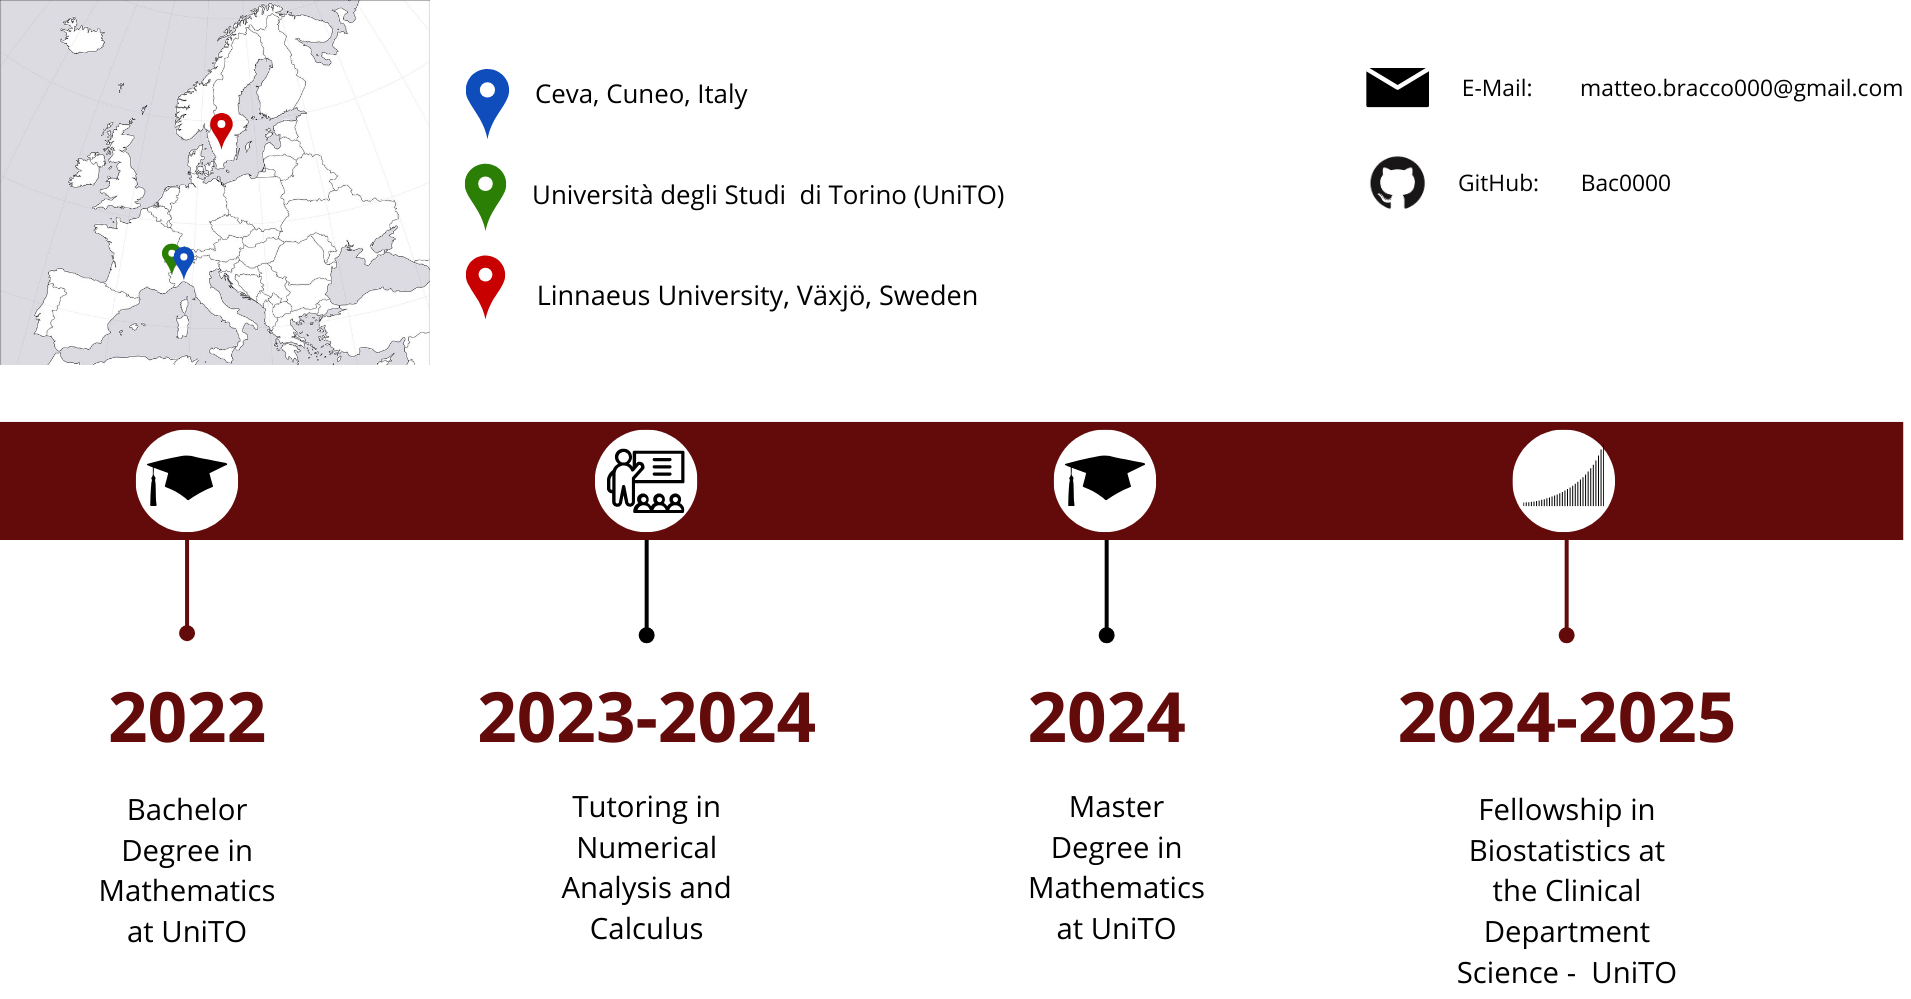
\includegraphics[width=\textwidth]{myself_1}
	\end{figure}
\end{frame}	

		\begin{frame}
	\frametitle{Introduction}
	\begin{figure}
		\centering
		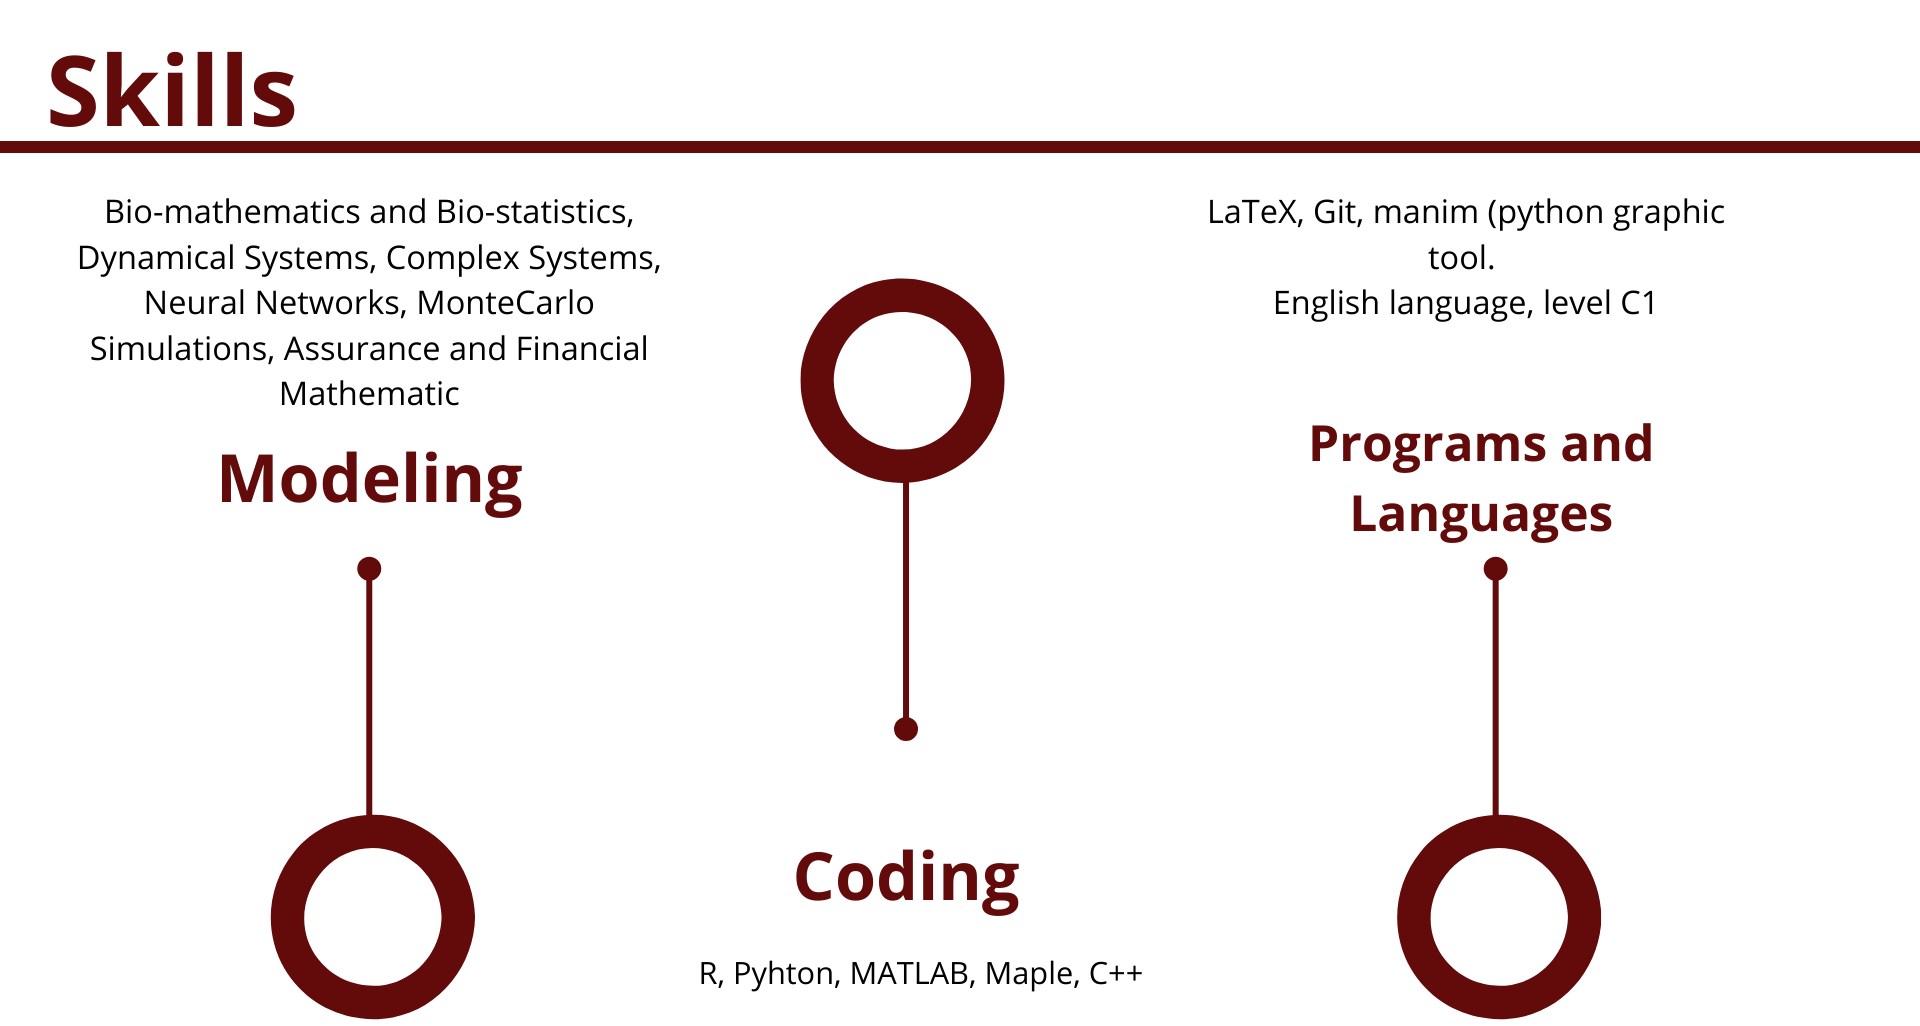
\includegraphics[width=\textwidth]{myself_2}
	\end{figure}
\end{frame}	
	
	\begin{frame}
		\frametitle{The SIR model}

		\begin{tikzpicture}[center coordinate=(box)]
			\node (A) at (3, 1) { \dftitle{Total Population: $N=S(t)+I(t)+R(t)$}{Bittersweet}};
			\node (C) at (0, 0) {\ball Infected ({\dftitle{I}{Gre}})};
			\node (D) at (3, 0) {\ball   Susceptibles ({\dftitle{S}{Gre}})};
			\node (E) at (6, 0)  {\ball   Removed ({\dftitle{R}{Gre}})};
			\node  (box) at (0,-3){%
			\begin{minipage}[c]{0.4\textwidth}
					\begin{figure}
						\centering
						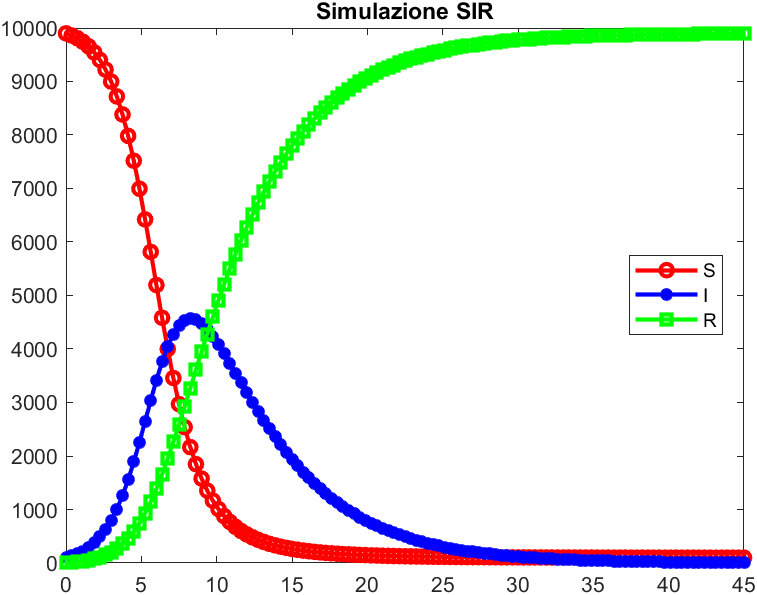
\includegraphics[width=5 cm]{SIR1} 
						\caption{Numeric Simulation of the SIR model}
					\end{figure}
				
				\end{minipage}
			};
			\node [ot] (box) at (6,-3.3){%
				\begin{minipage}[c]{0.4\textwidth}
					\centering
					{\deftitle{Model Equations}}
					$$
					\begin{cases}
						\dot S=-\frac{\beta}{N} S(t) I(t) \\
						\dot I= -\frac{\beta}{N} S(t) I(t)-\gamma I(t) \\
						\dot R= \gamma I(t)
					\end{cases}
					$$
					\begin{itemize}
						\item[\color{Gre}\cmark] {\dftitle{$\beta$}{Bittersweet}} is the infection rate  $I$  % per contatto I,S singolo
						\item[\color{Gre}\cmark] {\dftitle{$\gamma$}{Bittersweet}} $\propto$ $T^{-1}$ where $T$ is the average time of recovery from the illness.%in un unità di tempo
					\end{itemize}
				\end{minipage}
			};
		\end{tikzpicture}
	\end{frame} 
	
	
	\begin{frame}
		\frametitle{An Hidden Assumption}

	\begin{theorem}[Perfect Mixing]
		\centering
		$S$ and $I$ are uniformly distributed in space at all times
	\end{theorem}
\begin{figure}
	\centering
	\begin{minipage}{0.45\textwidth}
		\centering
		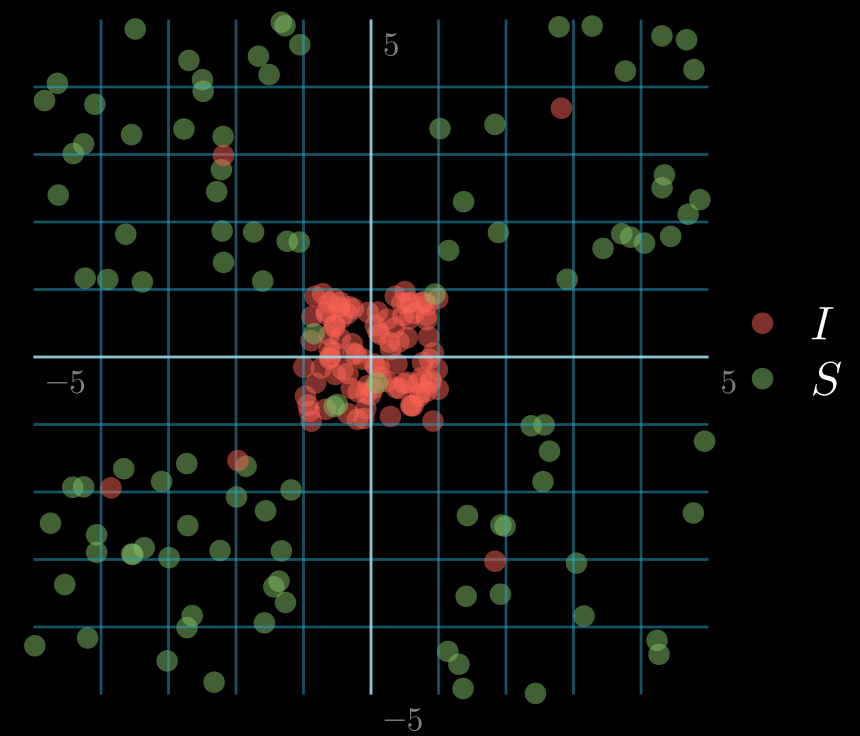
\includegraphics[width=4 cm]{dist1}
	\end{minipage}
	\begin{minipage}{0.45\textwidth}
		\centering
     	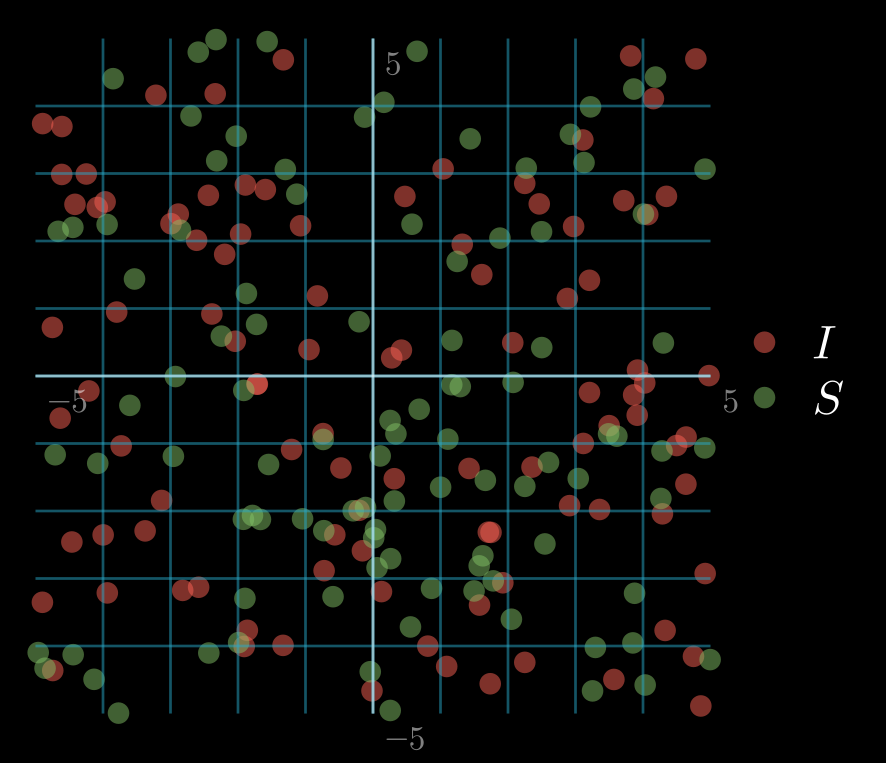
\includegraphics[width=4 cm]{dist2}
    \end{minipage}
	\caption{In the initial phases of an epidemic diffusion, the infected population $I$ is not uniformly spread across space}
\end{figure}
    	\end{frame}




\begin{frame}
	\frametitle{Lattice Gas Cellular Automata (LGCA)}
		\centering
	\begin{tikzpicture}
		\node  (box) at (0,0.8){%
			\begin{minipage}{0.8\textwidth}
				\centering
				{\dftitle{Particles and Cells}{Bittersweet}} \\
			\end{minipage}
		};
		\node [ot] (box) at (0,0){%
			\begin{minipage}{0.8\textwidth}
				\centering
			 Particles moving on a lattice can interact only inside the same cell
			\end{minipage}
		};
		
		
	\end{tikzpicture}
	\begin{figure}
		\centering
		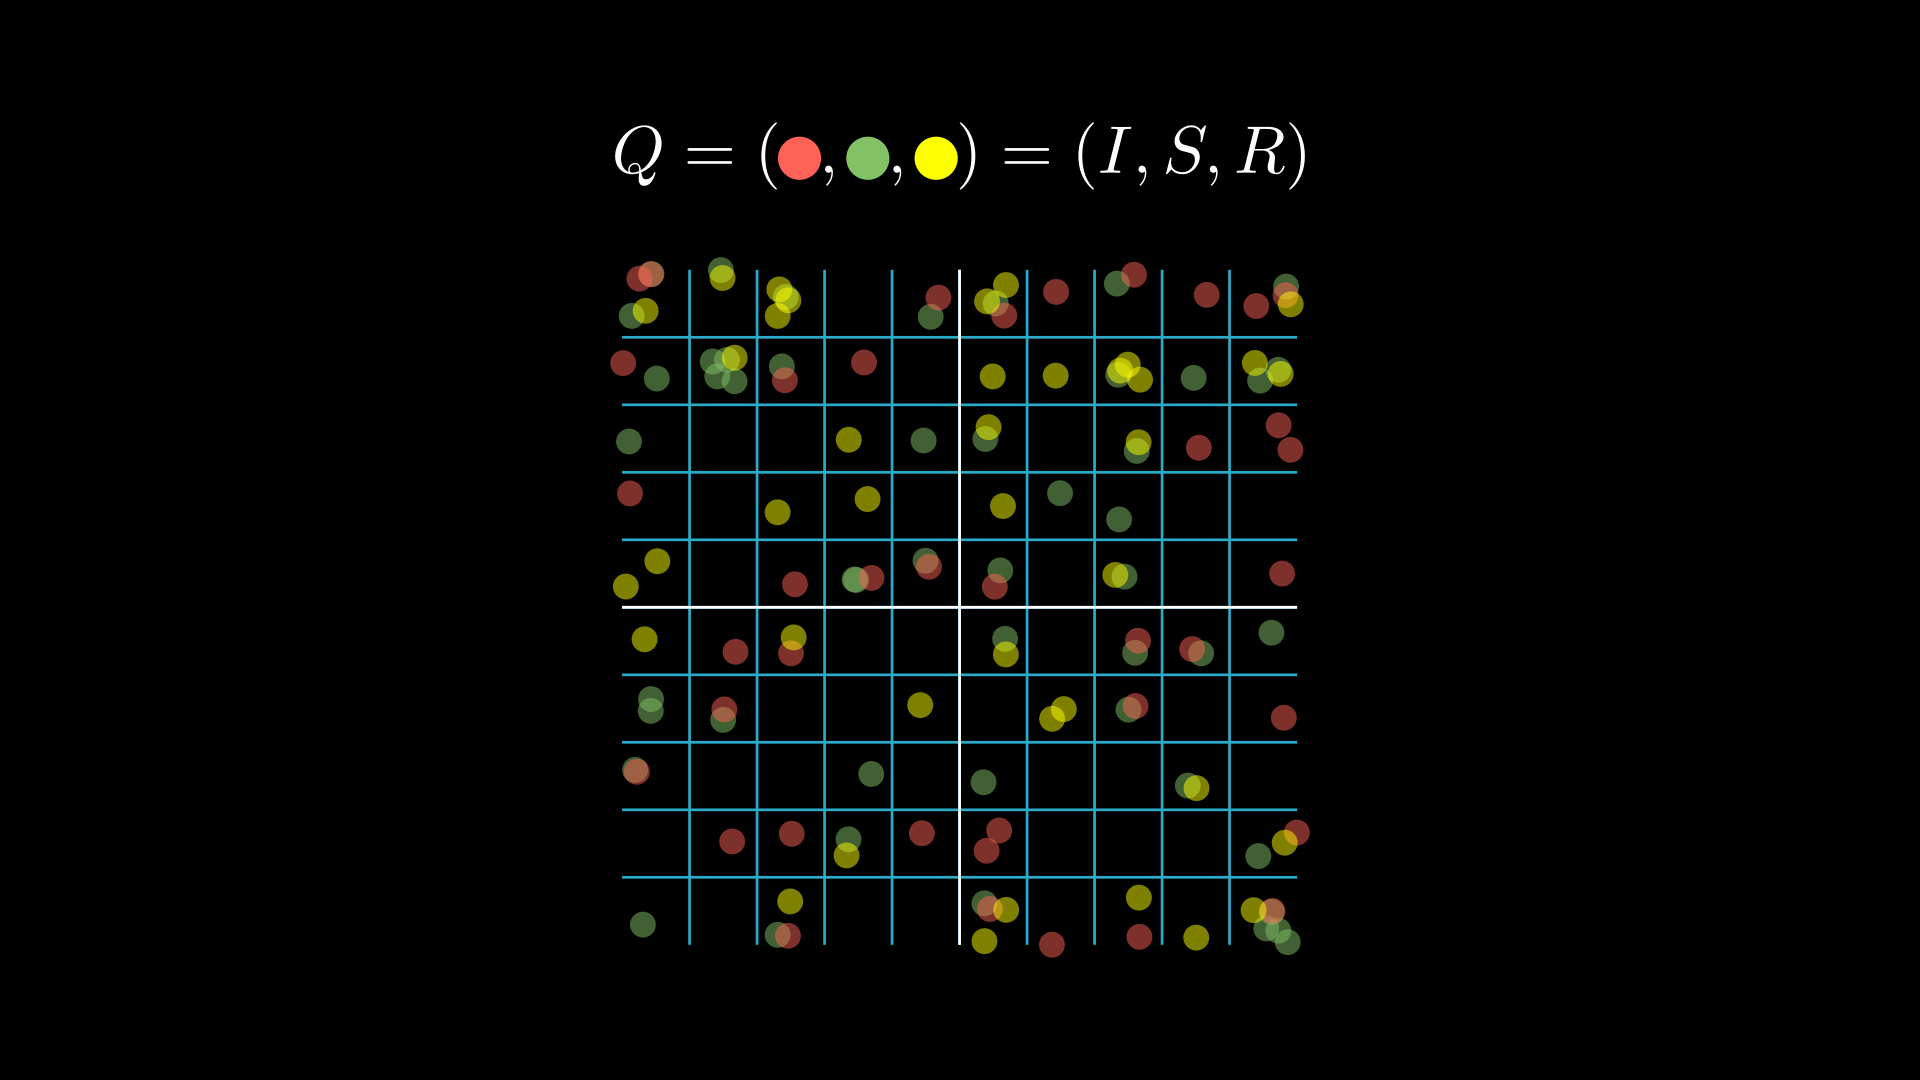
\includegraphics[width=0.9\linewidth]{lattice_states}
	\end{figure}
\end{frame}


\begin{frame}
	\frametitle{Particles Laws of Motion}
	\centering
	\begin{tikzpicture}
		\node  (box) at (0,0.9){%
			\begin{minipage}{0.95\textwidth}
				\centering
				{\dftitle{ At each time step $n$ particles move to a neighboor cell}{Bittersweet}} \\
			\end{minipage}
		};
			\node [ot] (box) at (-3,0){%
		\begin{minipage}{0.45\textwidth}
			\centering
			{\dftitle{Uniqueness}{Bittersweet}}\\
			
			 At most one particle can reach a fixed neighboor cell
		\end{minipage}
	};
			\node [ot] (box) at (3,0){%
	\begin{minipage}{0.45\textwidth}
		\centering
		{\dftitle{Randomnes}{Bittersweet}} \\
		
		 The exit configuration is randomly selected
	\end{minipage}
};
	\end{tikzpicture}

	\begin{figure}
		\centering
		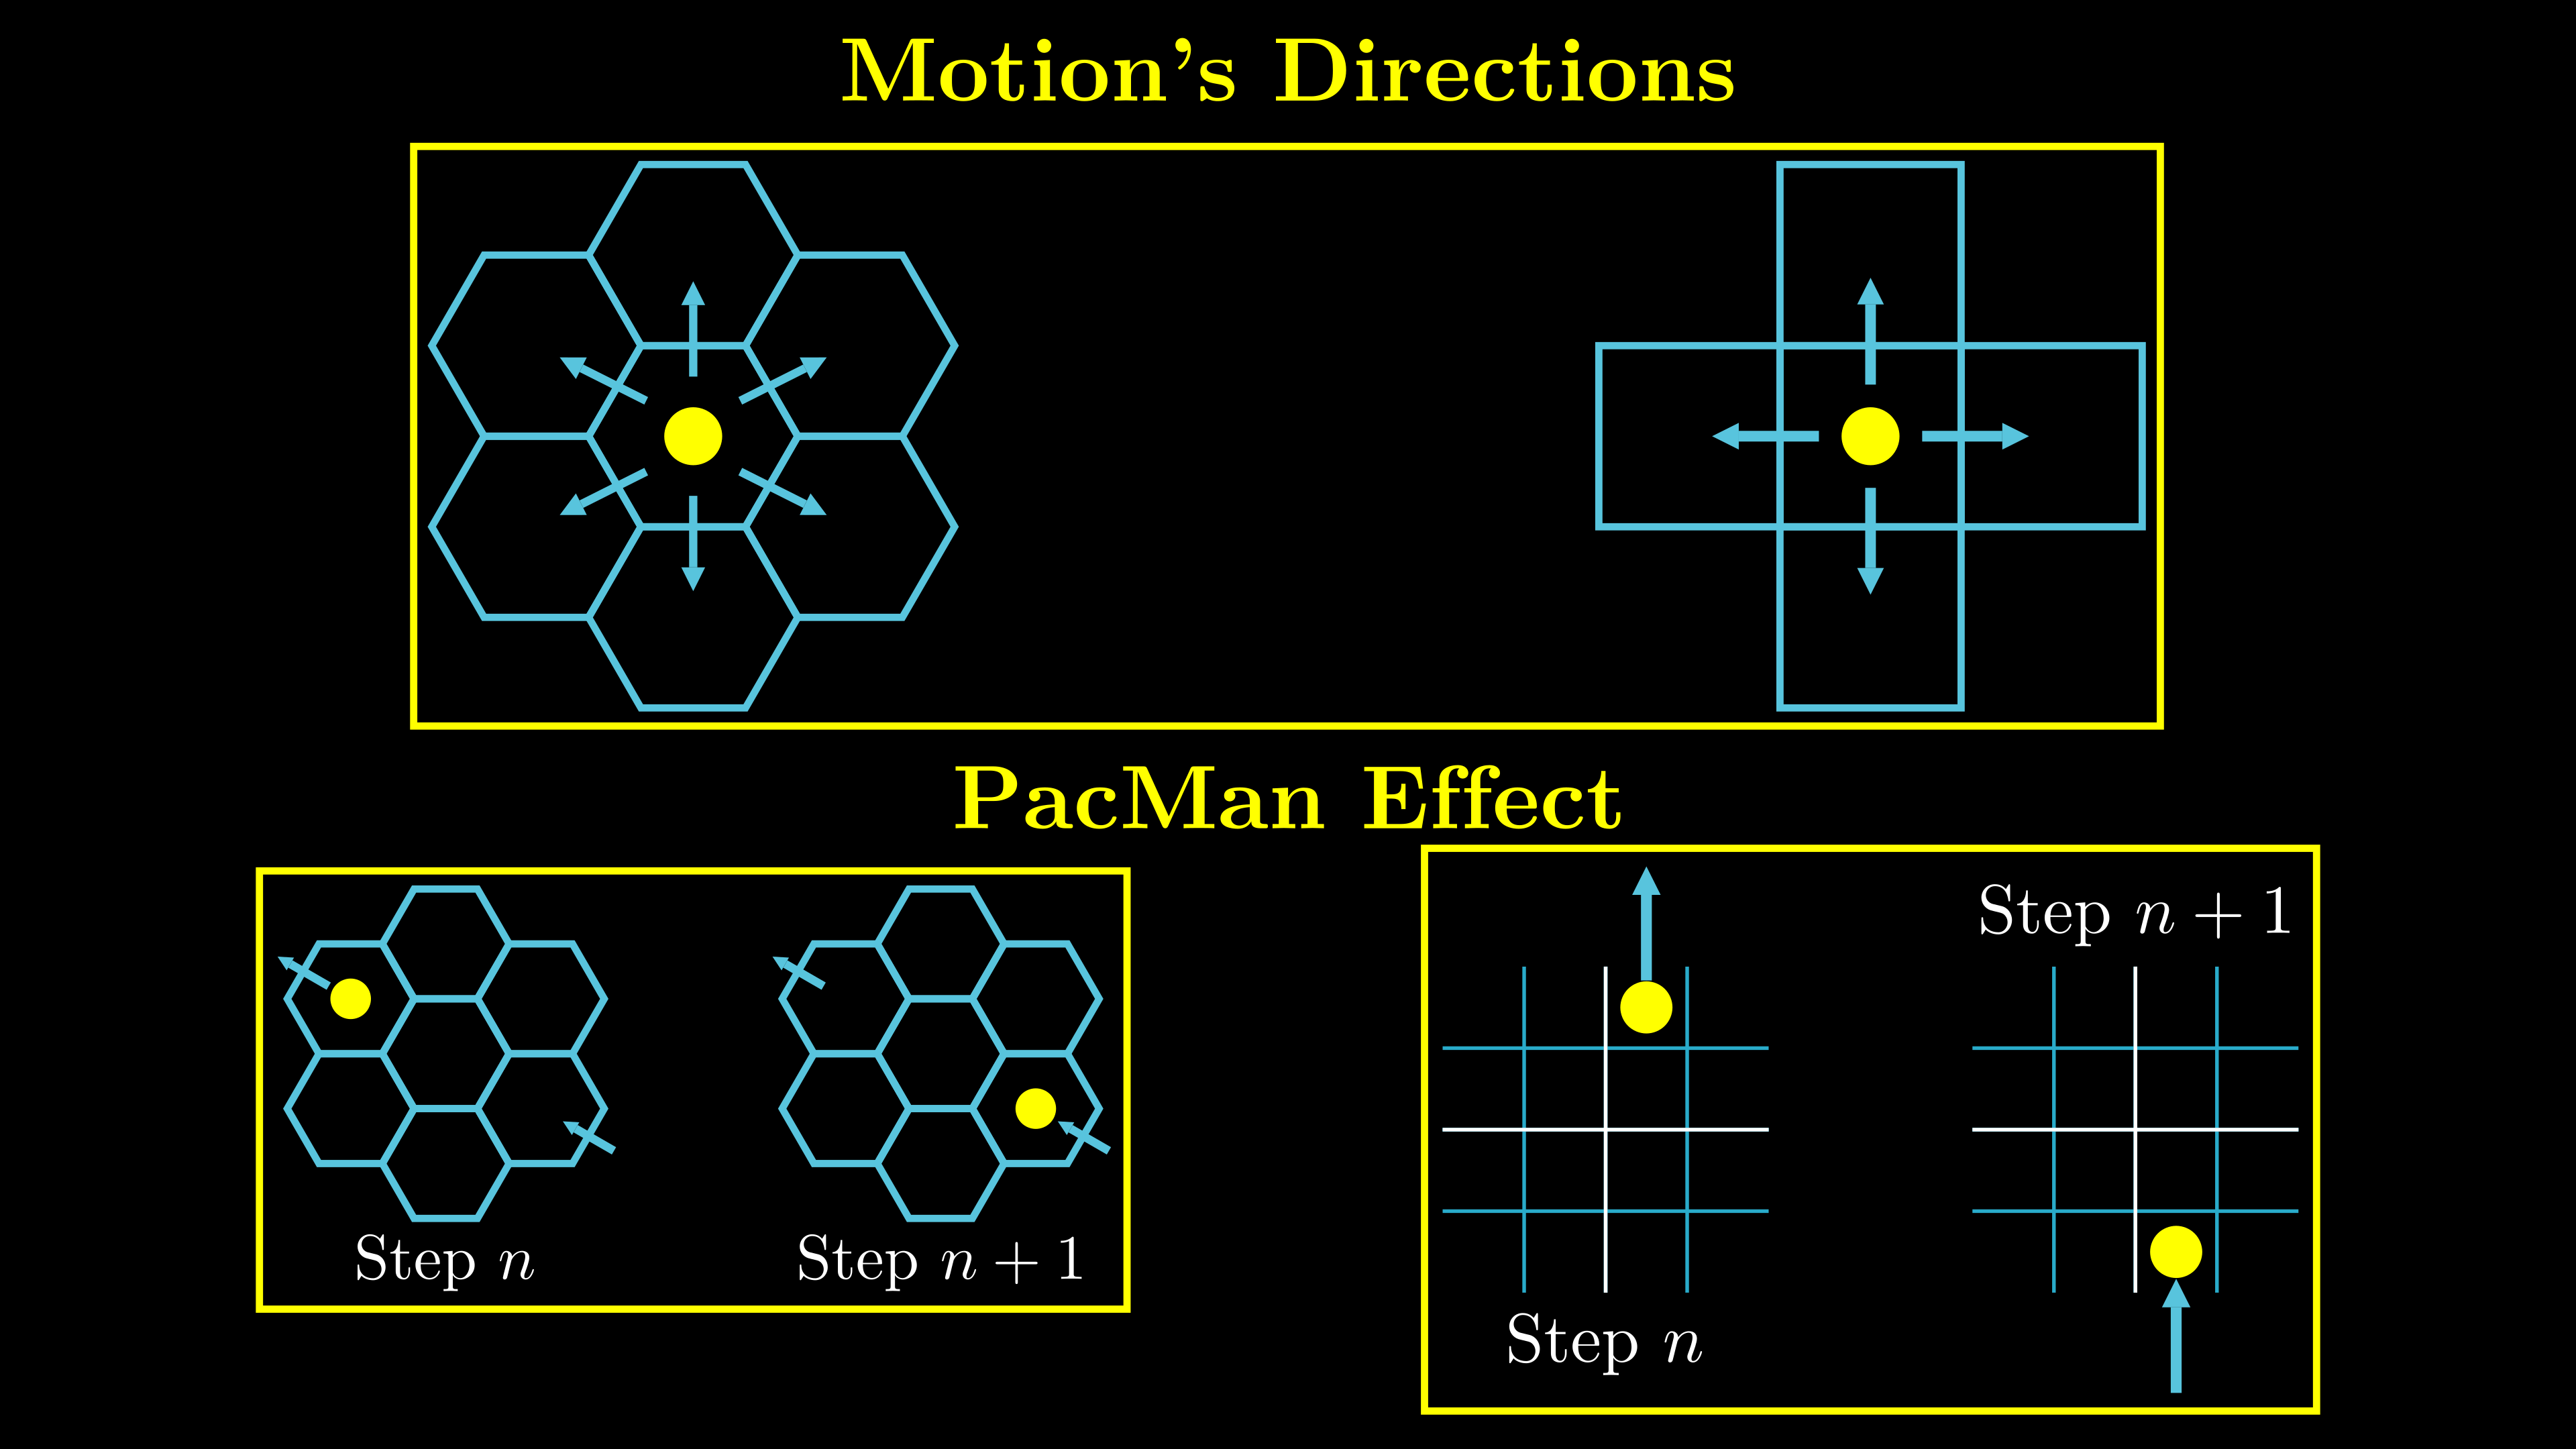
\includegraphics[width=0.8\linewidth]{moto}
	\end{figure}


\end{frame}

\begin{frame}
\frametitle{Epidemic Laws described}
\centering
		\begin{tikzpicture}
	
	\centering
	\node (box) at (0,1.5){%
		\deftitle{Evolution Rules}
	};
	\node [ot] (box) at (0,0){%
		\begin{minipage}{0.9\textwidth}
		\centering
		\begin{itemize}
		\item Each particle of state $I$ of a specific cell, infects a particle of state $S$ of the same cell with probability $\beta_{LG}$
		
		\item With rate $\gamma$ particles pass from state $I$ to state $R$
	\end{itemize}
	\end{minipage}
	};
\end{tikzpicture}
\begin{theorem}[Epidemic Laws inside a cell]
Let $I(c)$ be the number of infected in cell $c$ and let $q_n(p)$ be the state of particle $p \in c$ at time step $n$, then
\[
\begin{cases}
	 \phi_c=\p\left(q_{n+1}(p)=S |q_{n}(p)=S\right)=(1-\alpha_{LG})^{I(c)} \\
     \psi_c=\p\left(q_{n+1}(p)=I |q_{n}(p)=S\right)=1-\phi_c\\
     \p\left(q_{n+1}(p)=I |q_{n}(p)=I\right)=1-\beta_{LG} \\
     \p\left(q_{n+1}(p)=R |q_{n}(p)=I\right)=\beta_{LG}
\end{cases}
\]
\end{theorem}
\end{frame}


\begin{frame}
	\frametitle{Covid-19 in Kodiak Island, Alaska}
\begin{center}
	\dftitle{An overlook of data and estimated parameters}{Bittersweet}
\end{center}
	\begin{figure}
		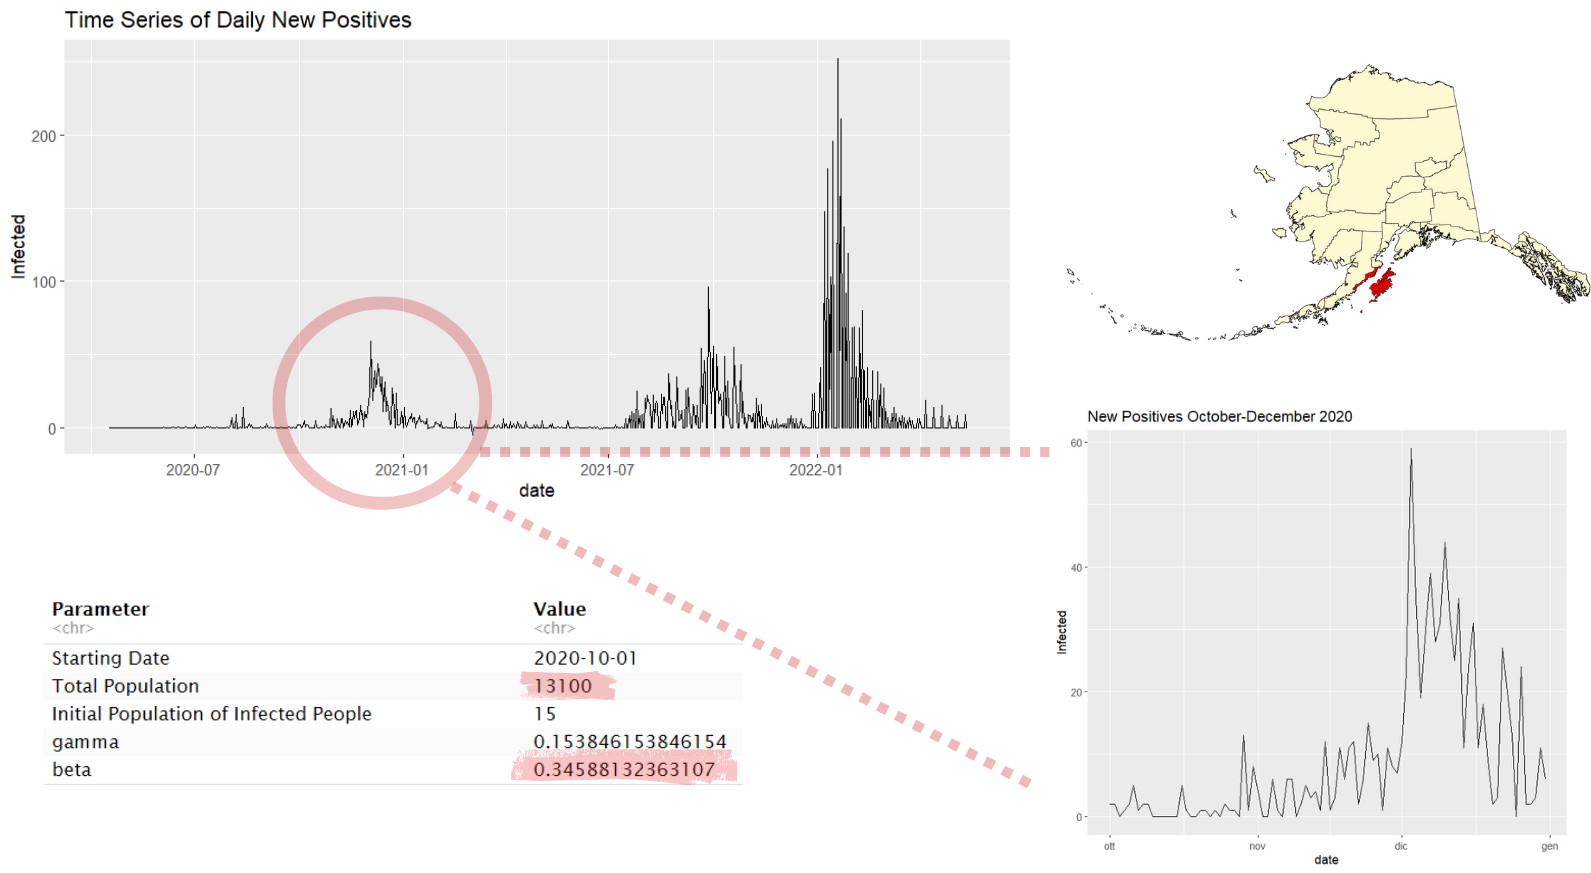
\includegraphics[width=0.93\linewidth]{covid_glob.png}
	\end{figure}

\end{frame}




\begin{frame}
	\frametitle{Covid-19 in Kodiak Island, Alaska}
\begin{center}
	\dftitle{How to estimate $\beta$ from new confirmed cases}{Bittersweet}
	\end{center}

	\begin{figure}
		\centering
		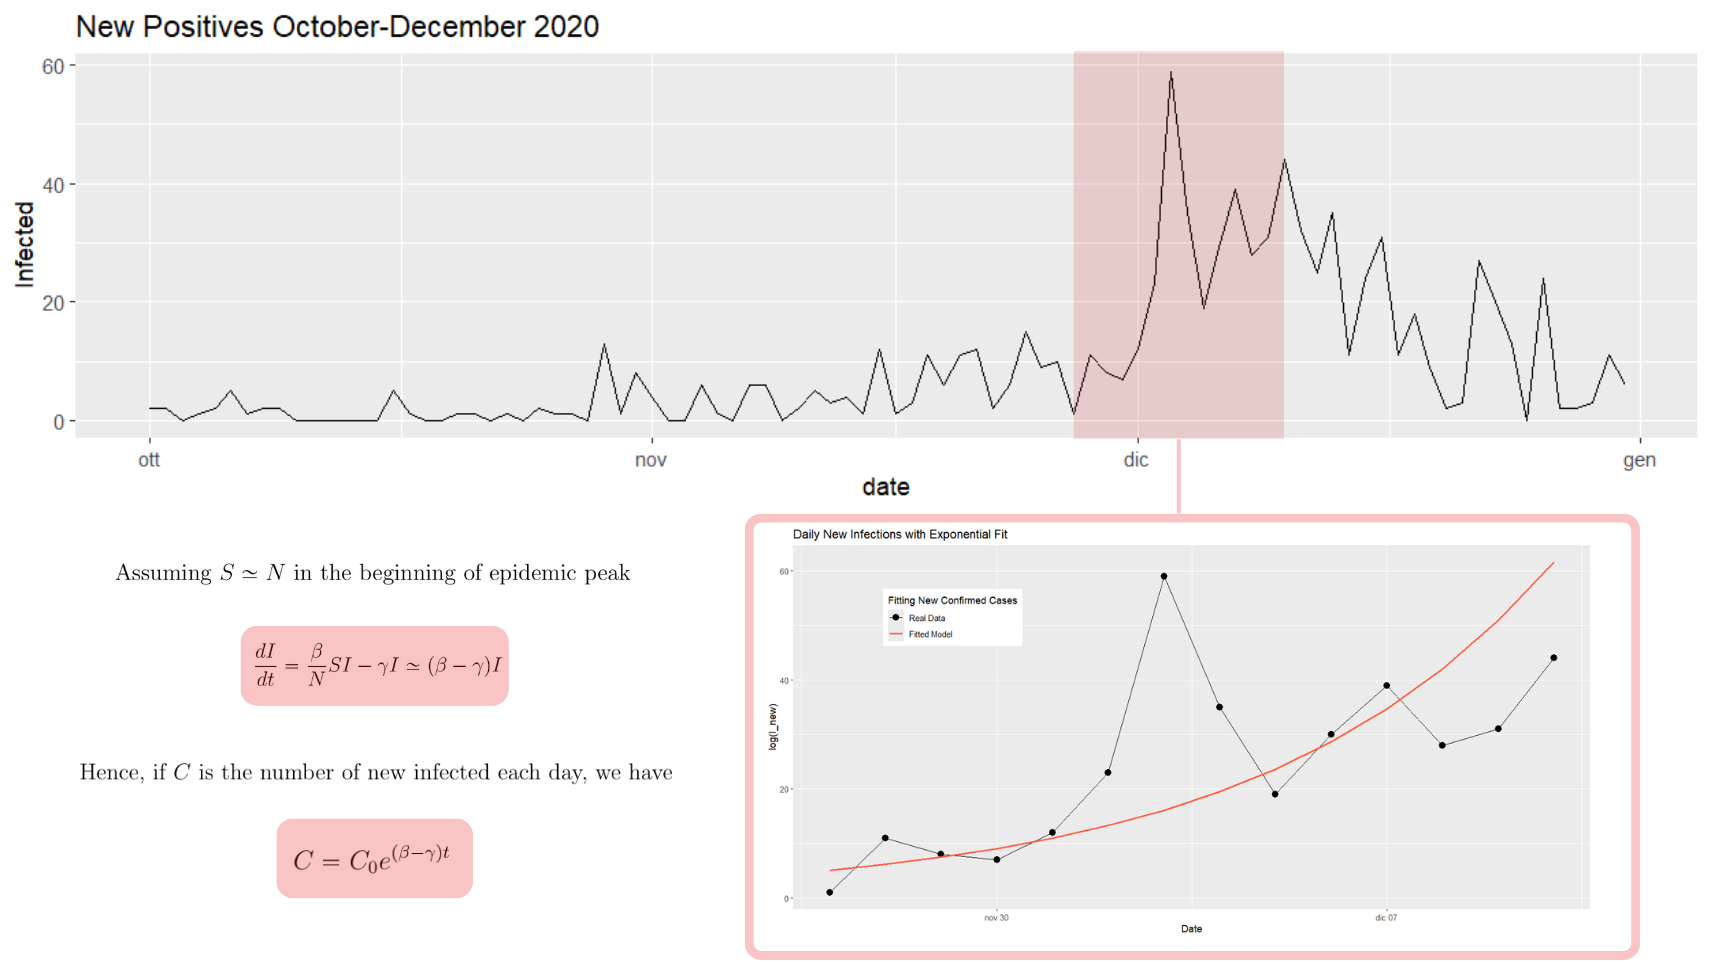
\includegraphics[width=0.95\linewidth]{beta_est}
	\end{figure}
\end{frame}

\begin{frame}
	\frametitle{Covid-19 in Kodiak Island, Alaska}
	\begin{center}
		\dftitle{SIR and LGCA Simulation Results}{Bittersweet}
	\end{center}
	\begin{figure}
		\centering
		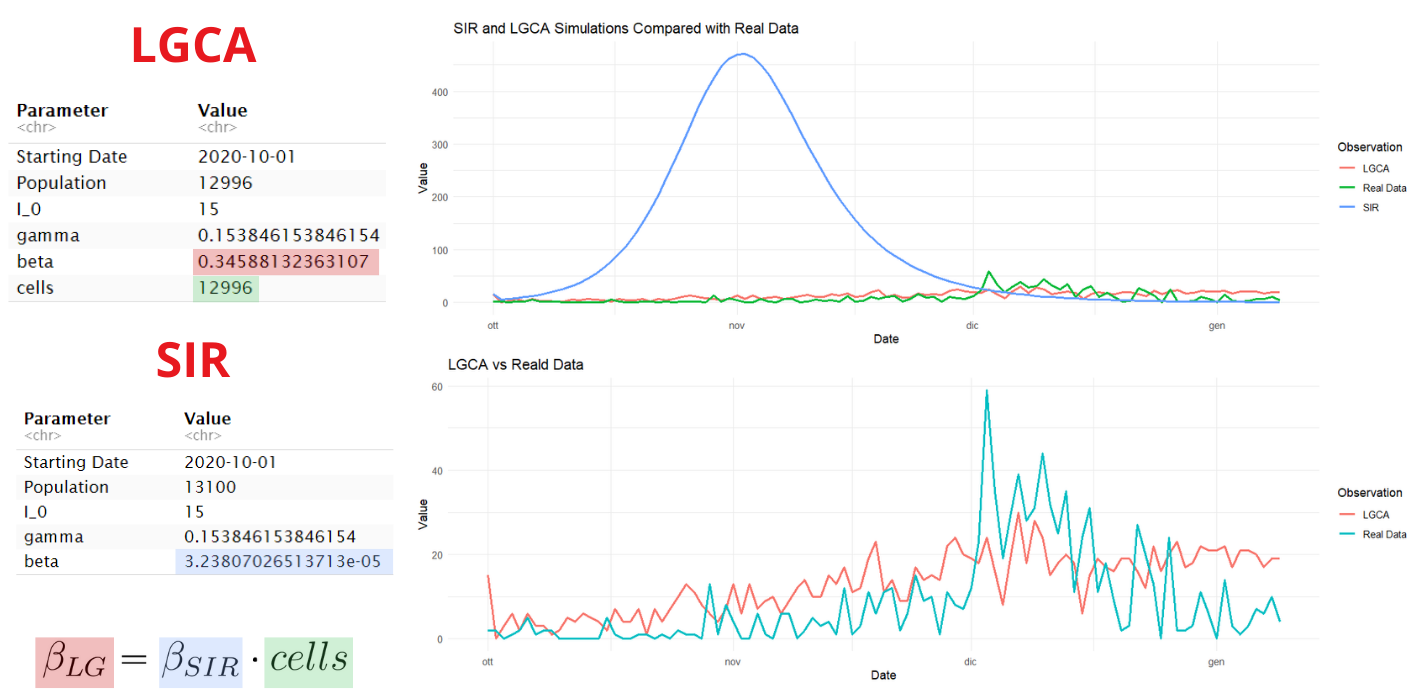
\includegraphics[width=0.95\linewidth]{Simul1_pres}
	\end{figure}
	
\end{frame}

\begin{frame}
	\frametitle{Modified LGCA algorithm}

		\begin{figure}
		\centering
		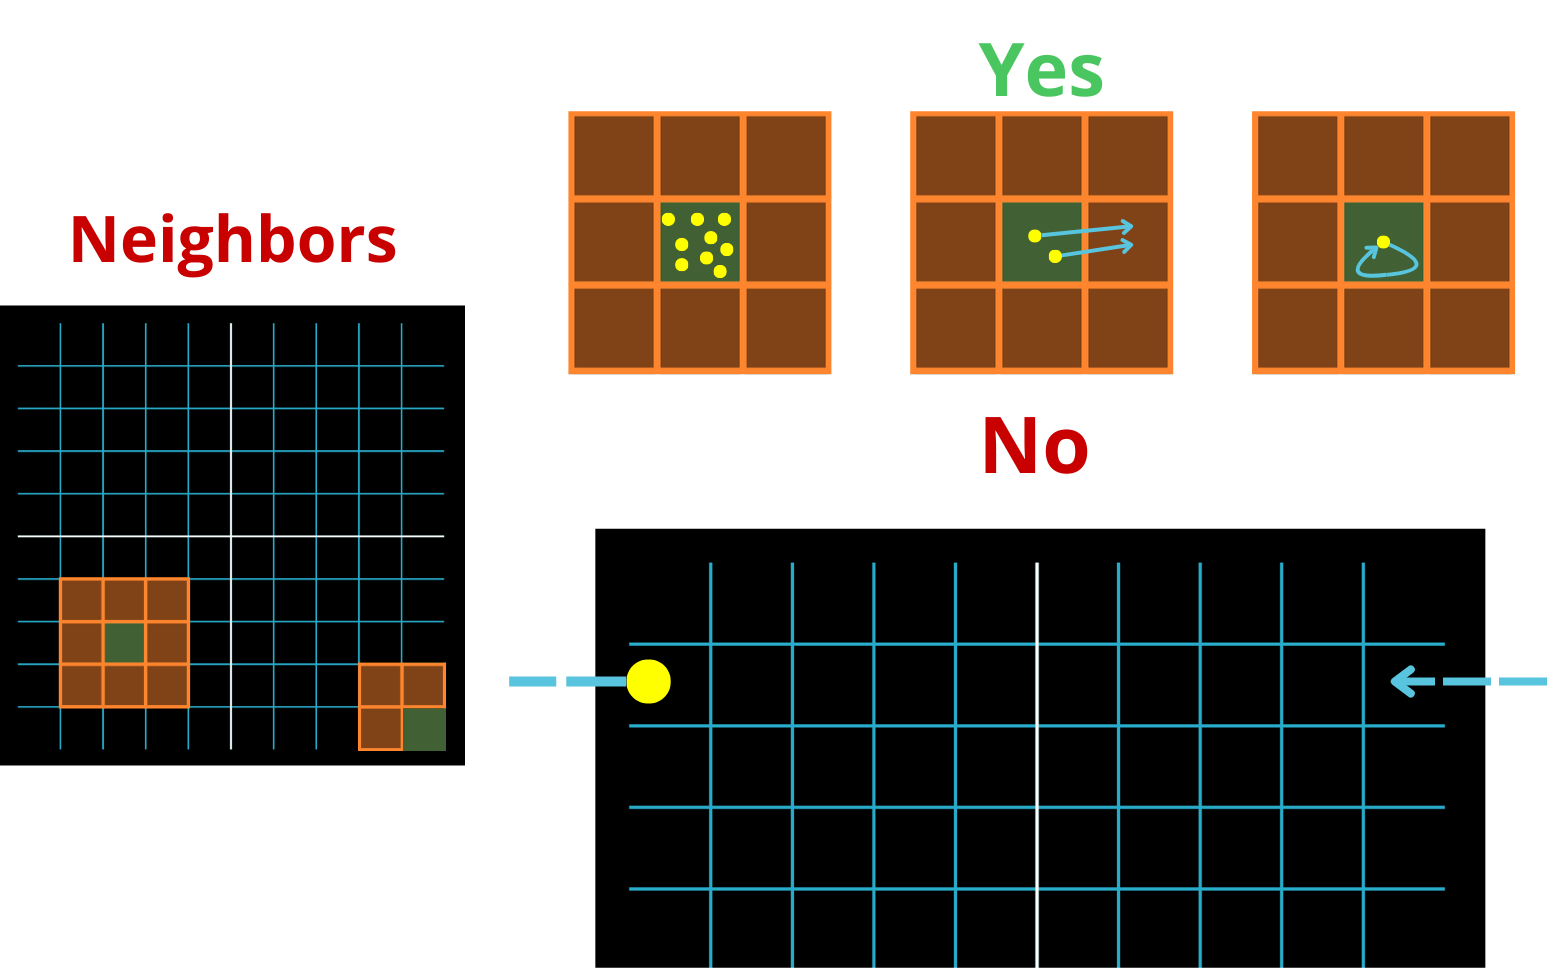
\includegraphics[width=0.9\linewidth]{modified_pres}
	\end{figure}
\end{frame}


\begin{frame}
	\frametitle{Modified LGCA Simulations}

		\begin{figure}
	\centering
	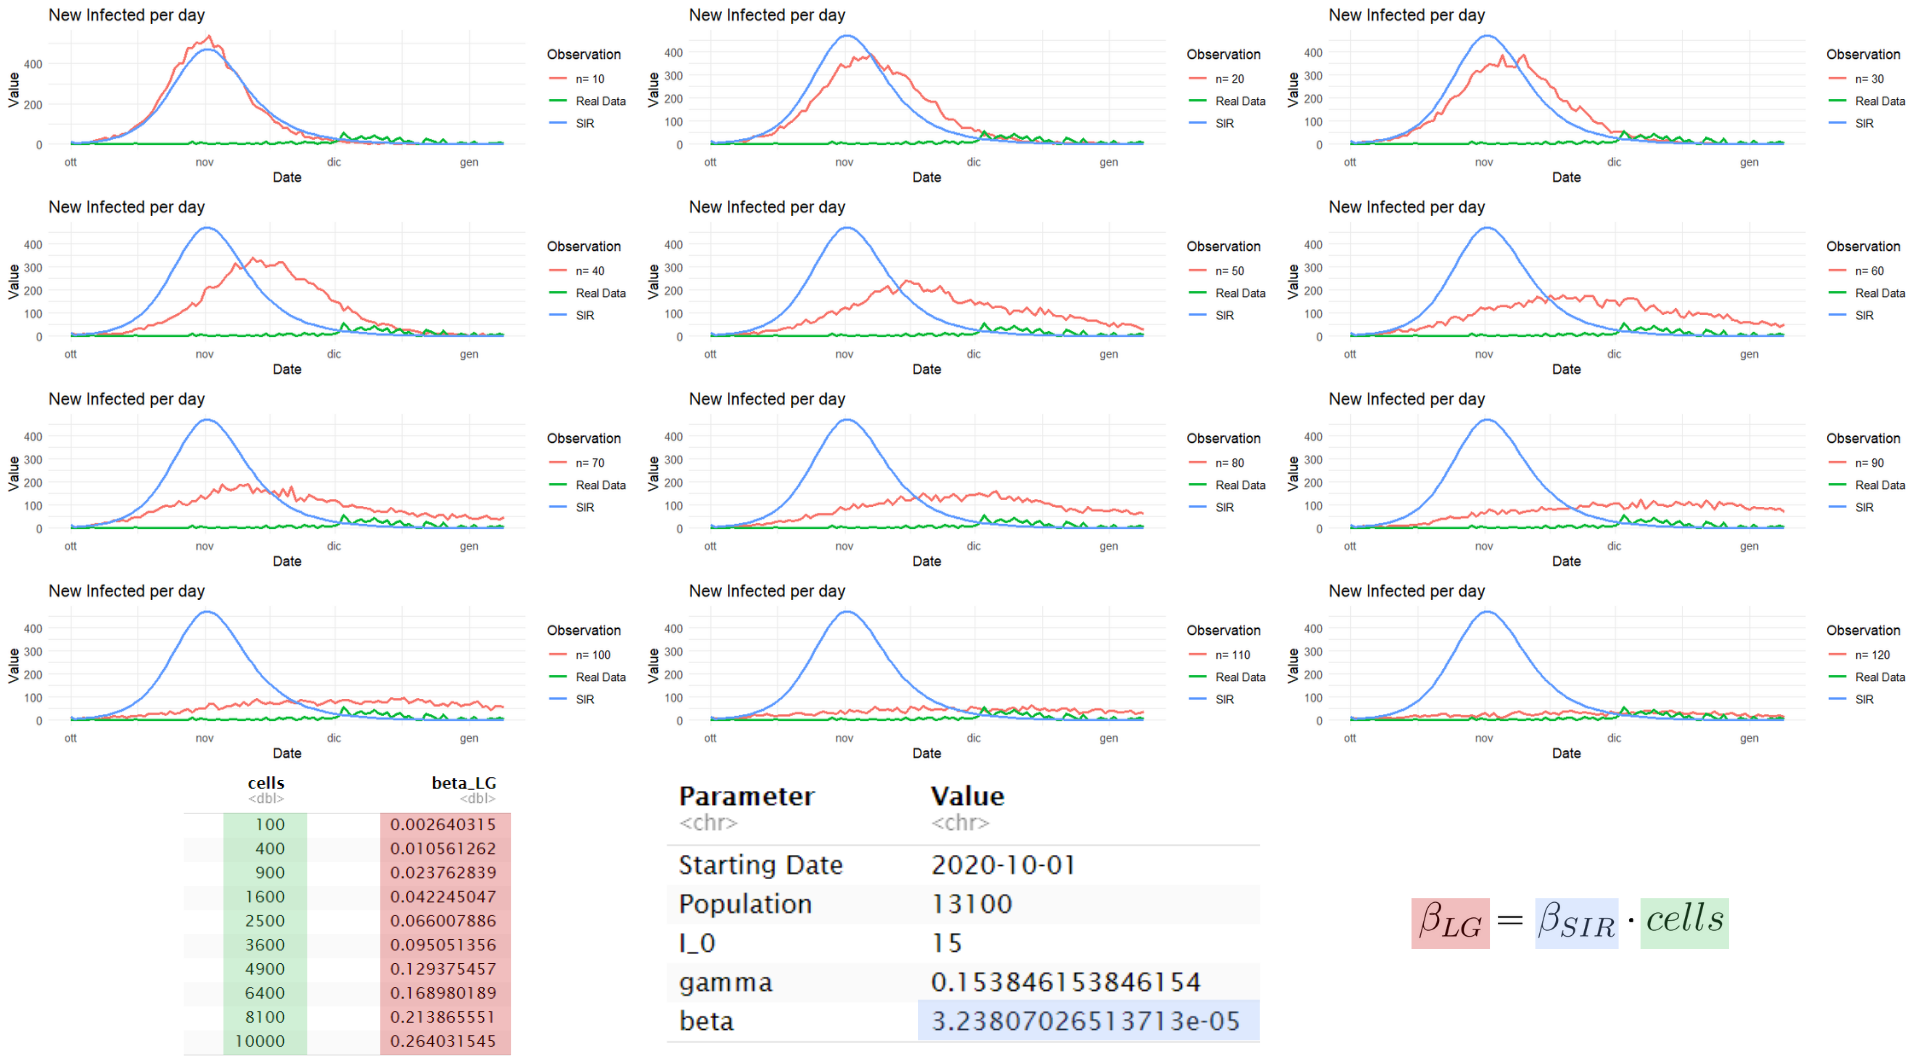
\includegraphics[width=0.95\linewidth]{MLGCA_withSIR}
\end{figure}
\end{frame}

\begin{frame}
	\frametitle{Modified LGCA Simulations}
	
	\begin{figure}
		\centering
		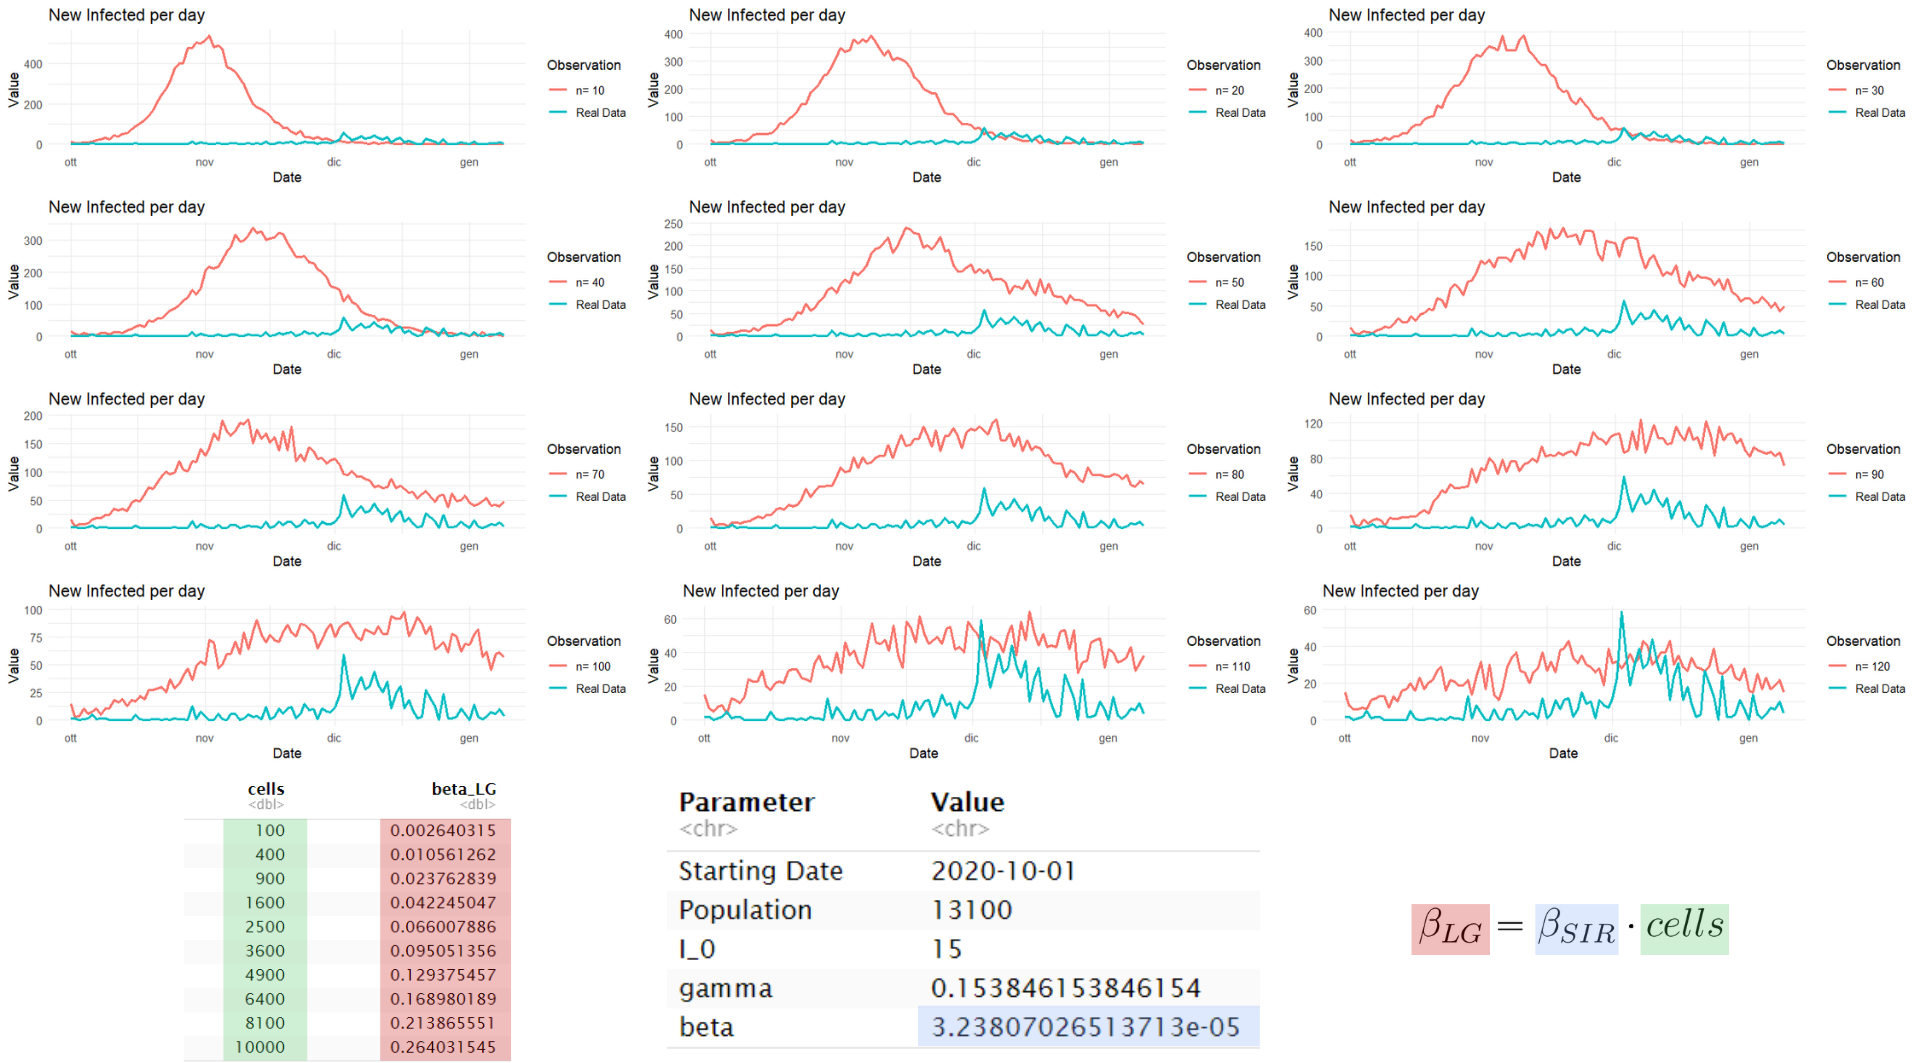
\includegraphics[width=0.95\linewidth]{MGCA_NOSIR}
	\end{figure}

\end{frame}

\begin{frame}
	\frametitle{Modified LGCA Simulations}
	
	\begin{figure}
		\centering
		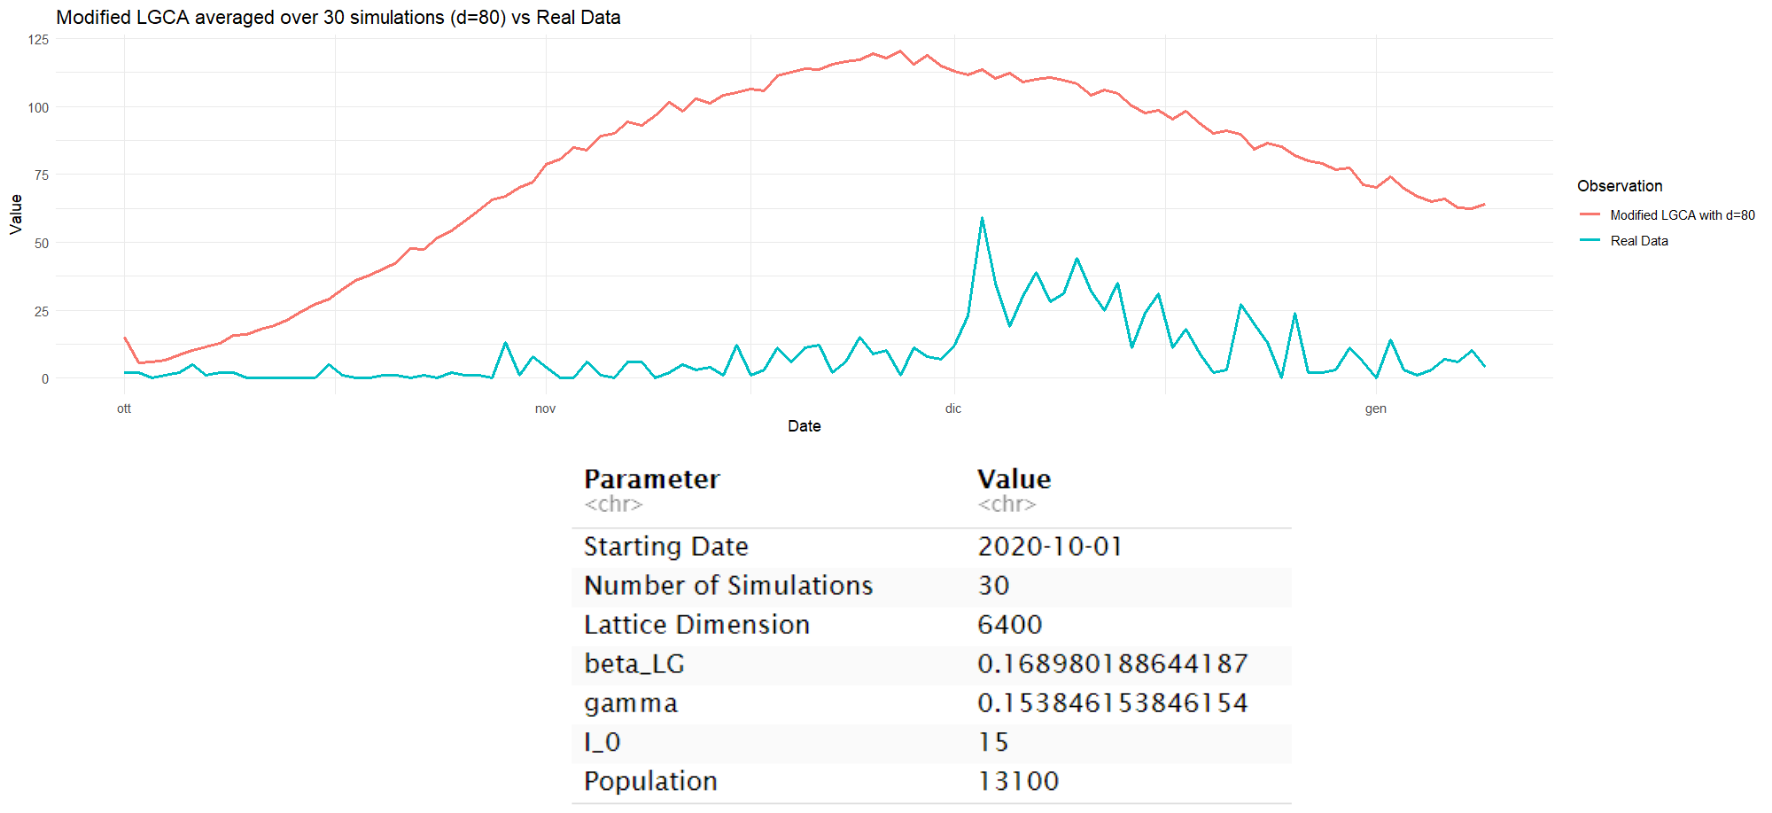
\includegraphics[width=0.95\linewidth]{Modmeans}
	\end{figure}
	
\end{frame}

 \begin{frame}

 	
 	\begin{figure}
 		\centering
 		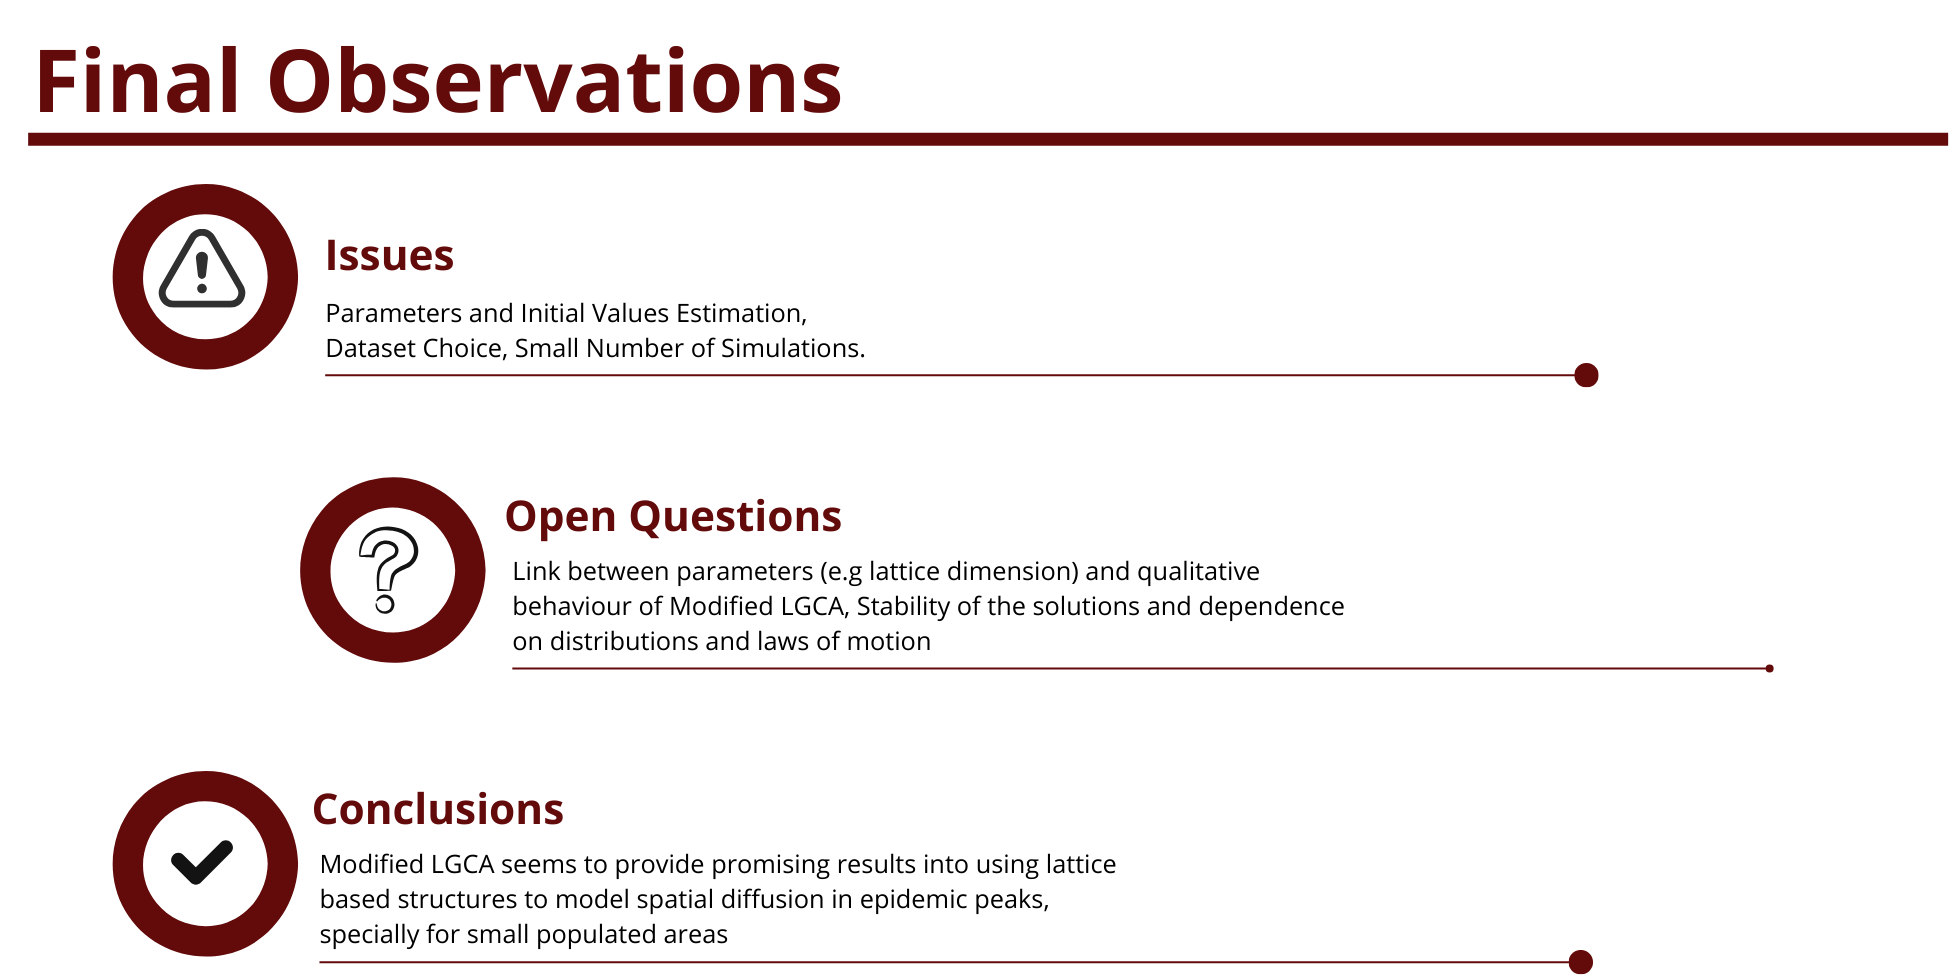
\includegraphics[width=0.95\linewidth]{conlusions_pres}
 	\end{figure}
 	
 \end{frame}
%			\begin{minipage}{0.4\textwidth}
%	\node (A) at (3, 1) { \dftitle{Ingredienti}{Bittersweet}};
%	\node (C) at (0, 0) 
%	\node (D) at (3, 0) {I vicini di ogni cella $\mathcal{N}(\alpha_i)$};
%	\node (E) at (6, 0)  {Un insieme finito $Q$ di stati che una cella può assumere};
%	\node (E) at (3, -1)  {Una regola deterministica $f$ che determina l'evoluzione del sistema};
%\end{minipage}
%};	
	
	\begin{frame}
		\frametitle{Bibliography}	
		\bibliographystyle{unsrt}
		\bibliography{pres_biblio.bib}
		\nocite{*}
		
		

\end{frame}
\end{document}